\section{Collaborative Filtering Model}
\label{sec:cf}
Model-based collaborative filtering for the user and recipes was applied. This approach utilizes information related to user ratings on the recipes. A Singular Value Decomposition algorithm has been applied to get the recommendations. The below approach was followed to get recommendations using SVD.

\begin{figure}[H]
	\centering
	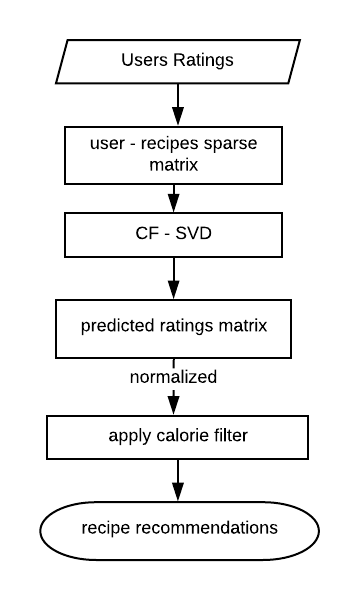
\includegraphics[width=0.5 \linewidth]{cf-svd}
	\caption{Collaborative Filtering- SVD Work-Flow }
	\label{fig:cf-svd}
\end{figure}  

\begin{itemize}
\item All user ids and recipe ids are extracted in such a way that every user id and recipe id represents a unique relationship via rating. The user id refers to unique id given to the user and recipe id refers to a unique id given to the recipe in the dataset. The matrix of user-recipes ratings is formed such as a user represents row and recipes represents columns. The cell value represents a rating for a recipe given by a user. From this matrix, the sparse matrix was created. 
\item The sparse matrix is the same as above matrix except it has high efficiency to perform large mathematical operations. To create a sparse matrix, 'csr\_matrix' function is used from 'scipy.sparse' library. The generated sparse matrix was sent as an input to the SVD algorithm.
\item SVD algorithm runs PCA on the user-rating matrix to give back factors of the rating matrix as discussed in \nameref{sec:svd}. The dot product of these factors returns a rating matrix with predicted ratings. 
\item Further, normalization was performed to get all predicted ratings for all users for all recipes.
\end{itemize}

\subsection{Experiment}
\label{sec:svd_exp}